\chapter{Container as a Service with Kubernetes}
\label{cha:caas}
Container as a Service (CaaS) is a term introduced by cloud providers, which provide a cloud based on demand container environment. But CaaS is more then just an on demand container environment like Docker, it provides orchestration and monitoring tooling for containers. Additionally, CaaS is considered to be a model for IT organizations and developers, how they can ship and run their applications anywhere. There are multiple CaaS providers on the market, but the most popular CaaS providers are Azure Container Service, Amazon Elastic Container Service for Kubernetes (Amazon EKS), and Google Kubernetes Engine, whereby they bring in their own flavor of CaaS, but all of them use Kubernetes beneath\cite{CNCFKubernetes2018, MicrosoftAzureAKS2018, AmazonWebServicesEKS2018, GoogleCloudKE2018}. \\

Kubernetes is a container orchestration platform for automating deployments, scaling, and operation of containers across a Kubernetes Cluster. Kubernetes has been invented by Google, is open source since 2015, and managed by the Cloud Native Computing Foundation (CNCF), whereby CNCF is under the umbrella of the Linux Foundation. Kubernetes has become the most popular container orchestration platform on the market and is used by many CaaS and PaaS providers\cite{CNCF2018}.

\section{The need for Container as a Service}
\label{sec:caas-need-for-caas}
Enterprises and developers face the need to dynamically adapt to workloads and to roll out new version of their services fast, and without any downtime. Applying dynamically to workloads requires a dynamic infrastructure, which is capable of scaling up when the workload increases, and scaling down when the workload decreases, which is non-trivial to be handled manually. Rolling out new versions without downtime require a well defined workflow, which ensures a well defined roll out behavior. For such uses cases, a CaaS platform like Kubernetes can be used. Kubernetes makes it possible to effortlessly manage complex service infrastructures, service scaling, and the roll out of services. Thus, complex service infrastructures become simple to implement and manage.
\newpage

Kubernetes provides a DSL, which allows to specify the desired state of the Kubernetes Cluster, as well as a automation tooling to interact with the Kubernetes Cluster. Kubernetes automatically ensures that the state of the Kubernetes Cluster meets its specification. Thus, the developers have only the need to specify the desired state of their Kubernetes Cluster. Kubernetes provides enterprises a platform for their services, which is effortlessly to specify and maintain via templates and the provided automation tooling, which makes Kubernetes an IaC tool as well, as discussed in Chapter \vref{cha:iac}. This makes it easy to modify the infrastructure at any time, which allows enterprises to apply to new requirements fast.

\section{Kubernetes}
\label{sec:caas-kubernetes}
Kubernetes is a CaaS platform to orchestrate containers in a cluster, whereby the Kubernetes Cluster nodes can be located in the cloud or in a dedicated data center. Kubernetes is designed as a client server architecture and a master slave architecture. At least one node in the Kubernetes Cluster acts as the Kubernetes Master, which is discussed in Section \vref{sec:caas-kubernetes-master}, and the other nodes in the Kubernetes Cluster act as the Kubernetes Workers, which are discussed in Section \vref{sec:caas-kubernetes-worker}. The Figure \ref{fig:kubernetes-cluster-architecture} illustrates the architecture of a Kubernetes Cluster.

\begin{figure}[htbp]
	\centering
	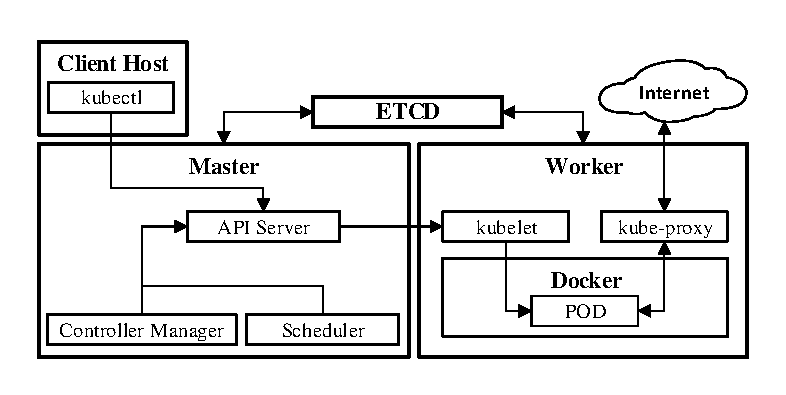
\includegraphics[scale=1]{images/kubernetes-cluster-architecture.pdf}
	\caption{Architecture of a Kubernetes Cluster}
	\label{fig:kubernetes-cluster-architecture}
\end{figure} 

\subsection{Kubernetes Objects}
\label{sec:caas-kubernetes-objects}
Kubernetes Objects are persistent objects in the Kubernetes System, and the Kubernetes Objects describe the state of the Kubernetes Cluster. The Kubernetes Cluster ensures that the state of the cluster meets the state specified by the Kubernetes Objects. The developers don't have to manually perform actions in the Kubernetes Cluster, they just have to modify the state represented by the Kubernetes Objects, and the Kubernetes Clusters itself will ensure that the modified state is applied on the Kubernetes Cluster. The following sections will briefly introduce some of the common used Kubernetes Objects. The overview of all Kubernetes Objects is covered by the Kubernetes API reference documentation\cite{CNCFKubernetesAPI2018}. 

\mysubsubsection{Pod}
A Pod is a group of one or more containers, which are managed together, and therefore share the same life-cycle. A Pod specification contains the specification for each container in the group. All of the containers of a Pod are always located on the same Kubernetes Worker, and will be deployed, started, and stopped as a single unit. In a pre-container world, all of the applications represented by the containers would have been hosted on the same physical machine. A Pod allows to bundle containers together, whereby the containers in a single Pod represent one instance of an  application\cite{CNCFKubernetesPods2018}. 

\mysubsubsection{Service}
A service is an abstraction, which defines a set of Pods and policies how to access them. The connection to the Pod, via the service abstraction, is handled by the Kubernetes Proxy. The service abstraction is necessary, because a Pod can be located on any Kubernetes Worker within the Kubernetes Cluster, and the Pod will therefore get a random IP assigned, which makes it impossible to address the Pod directly. If multiple replicas of a Pod are running, then the service will load balance the request between the Pods of the replica set, depending on the chosen algorithm\cite{CNCFKubernetesServices2018}.

\mysubsubsection{Secret}
A secret is an abstraction to manage sensitive configuration data, which can be consumed by containers. A secret holds a set of key value pairs, which represents the sensitive configuration data, and can be referenced by its name. A referenced secret can be injected into the container, either as a environment variable or a file. If the secret is injected as a file, then the filename represents the secret key and the file content represents the secret value. Developers reference secrets in the Pod specifications by their name, and only the referencing containers can access the injected sensitive configuration data the secret holds\cite{CNCFKubernetesSecrets2018}. 

\mysubsubsection{ConfigMap}
A configuration map works the same way as secrets, but is intended to hold non sensitive configuration data\cite{CNCFKubernetesConfigMap2018}.

\subsection{Kubernetes Master}
\label{sec:caas-kubernetes-master}
The Kubernetes Master is the master node in the Kubernetes Cluster, and is responsible for managing the Kubernetes Workers and Pods running on them. The Kubernetes Master exposes a REST API, via clients can interact with the Kubernetes Cluster. The node hosting the Kubernetes Master should be exclusively for the Kubernetes Master. The following sections briefly introduce the Kubernetes Master-Components, which are responsible for managing the Kubernetes Cluster\cite{CNCFKubernetesComponents2018}.

\mysubsubsection{Kubernetes CLI (kubectl)}
Kubectl is the CLI of Kubernetes, which provides an interface to manage the Kubernetes Cluster, and the Pods running on the Kubernetes Workers. Kubectl is similar to the Docker CLI, but does not support direct interacting with Docker. Kubectl interacts with the Kubernetes Cluster via the REST API exposed by the Kubernetes Master API-Server. Kubectl can be used from any client machine, which can connect to the cluster without any special setup.

\mysubsubsection{Distributed Key-Value Store (etcd)}
Etcd is a distributed key-value store, and provides a reliable way for sharing data within a cluster. It is the key component for the communication between the Kubernetes Masters and the Kubernetes Workers. The Kubernetes Master provides configuration for the Kubernetes Workers, and the Kubernetes Workers provide state information for the Kubernetes Master\cite{CoreOSETCD2018}.

\mysubsubsection{Kubernetes API-Server (kube-apiserver)}
The Kubernetes API-Server exposes the REST API for interacting with the Kubernetes Cluster, and is located on the Kubernetes Master. It represents the front-end of the Kubernetes Cluster and provides all necessary API to manage the Kubernetes Cluster, and the Kubernetes Objects.

\mysubsubsection{Kubernetes Scheduler (kube-scheduler)}
The Kubernetes Scheduler watches the Kubernetes Cluster for newly created Pods and assigns the Pods to a Kubernetes Worker. The Kubernetes Scheduler decides which Kubernetes Worker is suitable for the Pod. Multiple factors are taken into account for scheduling decisions such as, individual specifications, resource requirements, available resources, and hardware/policy/software constraints.

\mysubsubsection{Kubernetes Controller Manager (kube-controller-manager)}
The Kubernetes Controller Manager is responsible for managing the different controllers. A Kubernetes Controller is running in a loop and ensures that the state of the system is valid, depending on the controller type. For instance, the replication controller ensures the correct number of Pods for each replication controller object within the Kubernetes Cluster. Kubernetes provides a set of controllers such as, a replication controller, node controller, endpoint controller, and service account controller.

\subsection{Kubernetes Worker}
\label{sec:caas-kubernetes-worker}
The Kubernetes Worker is a node within the Kubernetes Cluster, which acts as the slave node, which runs the Pods, and is managed by the Kubernetes Master. The Kubernetes Worker can be a VM or a physical machine, depending on the Kubernetes Cluster setup. It contains the Kubernetes Runtime-Environment and used container runtime. The following sections briefly introduce the Kubernetes Worker-Components, which are responsible for running the Pods on the Kubernetes Worker\cite{CNCFKubernetesComponents2018}. 

\mysubsubsection{Kubernetes Agent (kubelet)}
The Kubernetes Agent is a process, running on the Kubernetes Worker, which interacts with the Kubernetes Master via its exposed REST API. The Kubernetes Agent ensures, that the containers are running in a Pod, as specified by the provided Pod specifications. The Pod specifications can be provided by a file in a specific directory, which gets periodically checked, or via the Kubernetes API-Server.

\mysubsubsection{Kubernetes Network-Proxy (kube-proxy)}
The Kubernetes Network-Proxy manages the networks defined by the specifications, and reflects the services, which are bound to a Pod. It can perform simple TCP and UDP forwarding, and can be connected to multiple back-ends. Any communication of a Pod to another Pod or to an external network is handled by the Kubernetes Network-Proxy. 

\mysubsubsection{Container Runtime}
The container runtime is the software responsible for running the containers on the Kubernetes Worker. Kubernetes supports multiple container runtimes, but mostly  Docker is used, which has been discussed in Chapter \vref{cha:containerization-docker}. \\

Kubernetes provides all features to implement a dynamic scalable service infrastructure such as, workflows for rolling out services, replica management, or secret and configuration management. Kubernetes is on top of the container runtime such as Docker, and provides orchestration tooling, necessary to run large scale containerized service infrastructures. Nevertheless, sometimes a pure container orchestration platform like Kubernetes is not enough, which for instances doesn't provides features for setting up a complete release workflow. This can be overcome with the usage of PaaS platforms like Openshift, which will be discussed in the following chapter.
